\documentclass[conference]{IEEEtran}

\usepackage{amsmath,amssymb}
\usepackage{booktabs}
\usepackage{graphicx}
\usepackage{multirow}
\usepackage{placeins}
\usepackage{url}

% Generated by tools/write_paper_result_macros.py; do not edit values manually.
\providecommand{\PMFCleanPSOMedian}{0.14823}
\providecommand{\PMFCleanCSMedian}{0.46803}
\providecommand{\PMFCleanPSOSuccess}{18/20}
\providecommand{\PMFCleanCSSuccess}{6/20}
\providecommand{\PMFCleanPSOWins}{18/20}
\providecommand{\PMFCleanWilcoxonP}{0.000322}
\providecommand{\PMFOutlierFiftyPSOMedian}{3.64209}
\providecommand{\PMFOutlierFiftyCSMedian}{3.44805}
\providecommand{\PMFOutlierFiftyPSOSuccess}{4/20}
\providecommand{\PMFOutlierFiftyCSSuccess}{1/20}
\providecommand{\PMFOutlierFiftyWilcoxonP}{0.349}
\providecommand{\SQOcclusionCenterFeasible}{5/9}
\providecommand{\SQOcclusionCenterInfeasible}{4/9}
\providecommand{\SupportCleanFullMedian}{0.14812}
\providecommand{\SupportCleanAdaptiveMedian}{0.17179}
\providecommand{\SupportCleanFullSuccess}{5/5}
\providecommand{\SupportCleanAdaptiveSuccess}{5/5}
\providecommand{\SupportCleanWilcoxonP}{0.062}
\providecommand{\SupportOutlierFiftyFullMedian}{3.54490}
\providecommand{\SupportOutlierFiftyAdaptiveMedian}{0.14828}
\providecommand{\SupportOutlierFiftyFullSuccess}{1/5}
\providecommand{\SupportOutlierFiftyAdaptiveSuccess}{5/5}
\providecommand{\SupportOutlierFiftyWilcoxonP}{0.125}
\providecommand{\SupportOutlierEightyFullMedian}{4.45124}
\providecommand{\SupportOutlierEightyAdaptiveMedian}{0.14886}
\providecommand{\SupportOutlierEightyFullSuccess}{0/5}
\providecommand{\SupportOutlierEightyAdaptiveSuccess}{5/5}
\providecommand{\SupportOutlierEightyWilcoxonP}{0.062}
\providecommand{\AreaBoxUniformMedian}{0.14372}
\providecommand{\AreaBoxWeightedMedian}{0.08296}
\providecommand{\AreaBoxUniformSuccess}{0/5}
\providecommand{\AreaBoxWeightedSuccess}{2/5}
\providecommand{\AreaEllipsoidUniformMedian}{0.02138}
\providecommand{\AreaEllipsoidWeightedMedian}{0.02083}
\providecommand{\AreaEllipsoidUniformSuccess}{4/5}
\providecommand{\AreaEllipsoidWeightedSuccess}{5/5}
\providecommand{\AreaCylinderUniformMedian}{0.07094}
\providecommand{\AreaCylinderWeightedMedian}{0.07426}
\providecommand{\AreaCylinderUniformSuccess}{0/5}
\providecommand{\AreaCylinderWeightedSuccess}{1/5}
\providecommand{\InitBoxRandomMedian}{0.08184}
\providecommand{\InitBoxGuidedMedian}{0.02791}
\providecommand{\InitBoxRandomSuccess}{1/5}
\providecommand{\InitBoxGuidedSuccess}{5/5}
\providecommand{\InitCylinderRandomMedian}{0.07345}
\providecommand{\InitCylinderGuidedMedian}{0.02946}
\providecommand{\InitCylinderRandomSuccess}{1/5}
\providecommand{\InitCylinderGuidedSuccess}{5/5}
\providecommand{\InitEllipsoidRandomMedian}{0.02006}
\providecommand{\InitEllipsoidGuidedMedian}{0.02010}
\providecommand{\InitEllipsoidRandomSuccess}{5/5}
\providecommand{\InitEllipsoidGuidedSuccess}{5/5}
\providecommand{\SQIndependentCases}{30}
\providecommand{\SQRunsPerCondition}{90}
\providecommand{\SQRandomPSOMedian}{0.03660}
\providecommand{\SQRandomPSOSuccess}{73/90}
\providecommand{\SQRandomEMSMedian}{0.02718}
\providecommand{\SQRandomEMSSuccess}{30/30}
\providecommand{\SQRandomEMSWins}{29/30}
\providecommand{\SQRandomWilcoxonP}{8.01\times10^{-8}}
\providecommand{\EMSOcclusionMedian}{0.03022}
\providecommand{\EMSOcclusionSuccess}{21/30}
\providecommand{\EMSOcclusionRuntime}{0.365}
\providecommand{\SQNoisePSOMedian}{0.04833}
\providecommand{\SQNoisePSOSuccess}{51/90}
\providecommand{\SQNoisePSOSuccessAtSix}{63/90}
\providecommand{\SQNoiseEMSMedian}{0.02793}
\providecommand{\SQNoiseEMSSuccess}{30/30}
\providecommand{\SQNoiseRelativeDegradation}{0.277}
\providecommand{\SQNoiseSmoothSuccess}{30/30}
\providecommand{\SQNoiseMixedSuccess}{10/30}
\providecommand{\SQNoiseBoxySuccess}{11/30}
\providecommand{\SQNoisePairedCleanP}{1.99\times10^{-6}}
\providecommand{\SQNoisePSOvsEMSP}{3.73\times10^{-9}}
\providecommand{\SQOutlierPSOMedian}{0.03687}
\providecommand{\SQOutlierPSOSuccess}{65/90}
\providecommand{\SQOutlierPSOSuccessAtSix}{80/90}
\providecommand{\SQOutlierEMSMedian}{0.02715}
\providecommand{\SQOutlierEMSSuccess}{30/30}
\providecommand{\SQOutlierRelativeDegradation}{0.030}
\providecommand{\SQOutlierSmoothSuccess}{30/30}
\providecommand{\SQOutlierMixedSuccess}{13/30}
\providecommand{\SQOutlierBoxySuccess}{22/30}
\providecommand{\SQOutlierPairedCleanP}{0.001131}
\providecommand{\SQOutlierPSOvsEMSP}{1.86\times10^{-9}}
\providecommand{\SQRandomMissingPSOMedian}{0.04568}
\providecommand{\SQRandomMissingPSOSuccess}{56/90}
\providecommand{\SQRandomMissingPSOSuccessAtSix}{69/90}
\providecommand{\SQRandomMissingEMSMedian}{0.02709}
\providecommand{\SQRandomMissingEMSSuccess}{29/30}
\providecommand{\SQRandomMissingRelativeDegradation}{0.142}
\providecommand{\SQRandomMissingSmoothSuccess}{30/30}
\providecommand{\SQRandomMissingMixedSuccess}{10/30}
\providecommand{\SQRandomMissingBoxySuccess}{16/30}
\providecommand{\SQRandomMissingPairedCleanP}{1.86\times10^{-9}}
\providecommand{\SQRandomMissingPSOvsEMSP}{1.86\times10^{-9}}
\providecommand{\SQOcclusionPSOMedian}{0.92729}
\providecommand{\SQOcclusionPSOSuccess}{0/90}
\providecommand{\SQOcclusionPSOSuccessAtSix}{0/90}
\providecommand{\SQOcclusionEMSMedian}{0.03022}
\providecommand{\SQOcclusionEMSSuccess}{21/30}
\providecommand{\SQOcclusionRelativeDegradation}{26.355}
\providecommand{\SQOcclusionSmoothSuccess}{0/30}
\providecommand{\SQOcclusionMixedSuccess}{0/30}
\providecommand{\SQOcclusionBoxySuccess}{0/30}
\providecommand{\SQOcclusionPairedCleanP}{1.86\times10^{-9}}
\providecommand{\SQOcclusionPSOvsEMSP}{1.86\times10^{-9}}
\providecommand{\BudgetFiftyKCleanPSOMedian}{0.14785}
\providecommand{\BudgetFiftyKCleanCSMedian}{0.32274}
\providecommand{\BudgetFiftyKCleanPSOSuccess}{5/5}
\providecommand{\BudgetFiftyKCleanCSSuccess}{2/5}
\providecommand{\BudgetFiftyKCleanPSOvsCSP}{0.062}
\providecommand{\BudgetFiftyKOutlierFiftyPSOMedian}{0.33920}
\providecommand{\BudgetFiftyKOutlierFiftyCSMedian}{3.38978}
\providecommand{\BudgetFiftyKOutlierFiftyPSOSuccess}{2/5}
\providecommand{\BudgetFiftyKOutlierFiftyCSSuccess}{0/5}
\providecommand{\BudgetFiftyKOutlierFiftyPSOvsCSP}{0.312}
\providecommand{\BudgetTwoHundredKCleanPSOMedian}{0.14816}
\providecommand{\BudgetTwoHundredKCleanCSMedian}{0.22376}
\providecommand{\BudgetTwoHundredKCleanPSOSuccess}{5/5}
\providecommand{\BudgetTwoHundredKCleanCSSuccess}{3/5}
\providecommand{\BudgetTwoHundredKCleanPSOvsCSP}{0.062}
\providecommand{\BudgetTwoHundredKOutlierFiftyPSOMedian}{0.33920}
\providecommand{\BudgetTwoHundredKOutlierFiftyCSMedian}{0.76300}
\providecommand{\BudgetTwoHundredKOutlierFiftyPSOSuccess}{2/5}
\providecommand{\BudgetTwoHundredKOutlierFiftyCSSuccess}{0/5}
\providecommand{\BudgetTwoHundredKOutlierFiftyPSOvsCSP}{0.625}
\providecommand{\BudgetFiveHundredKCleanPSOMedian}{0.14823}
\providecommand{\BudgetFiveHundredKCleanCSMedian}{0.18794}
\providecommand{\BudgetFiveHundredKCleanPSOSuccess}{5/5}
\providecommand{\BudgetFiveHundredKCleanCSSuccess}{3/5}
\providecommand{\BudgetFiveHundredKCleanPSOvsCSP}{0.062}
\providecommand{\BudgetFiveHundredKOutlierFiftyPSOMedian}{0.33920}
\providecommand{\BudgetFiveHundredKOutlierFiftyCSMedian}{0.38637}
\providecommand{\BudgetFiveHundredKOutlierFiftyPSOSuccess}{2/5}
\providecommand{\BudgetFiveHundredKOutlierFiftyCSSuccess}{2/5}
\providecommand{\BudgetFiveHundredKOutlierFiftyPSOvsCSP}{1.000}
\providecommand{\BudgetCleanPSOEndpointP}{0.625}
\providecommand{\BudgetCleanCSEndpointP}{0.438}
\providecommand{\BudgetOutlierFiftyPSOEndpointP}{0.312}
\providecommand{\BudgetOutlierFiftyCSEndpointP}{0.062}

% Character fitting results consolidated from the audited 2026-07-23 runs.
% Matched fitting: outputs/character_pso_cs_matrix_20260723/summary.json
% Four-way pilot: outputs/character_four_way_formal_20260723/manifest.json
% Guided PSO: outputs/character_pso_guided_fix_20260723 and
%             outputs/character_guided_pso_four_way_remaining_20260723
% Repeats 2--3: outputs/character_four_way_repeated_3seeds_20260723/manifest.json
% Guided CS: outputs/character_four_way_guided_cs_3seeds_20260727/manifest.json
% Ten-case factorial:
% outputs/character_matched_factorial_10cases_3seeds_20260727/summary/summary.json
\providecommand{\CharacterMatchedCases}{10}
\providecommand{\CharacterPSOSimilarityMedian}{66.48}
\providecommand{\CharacterCSSimilarityMedian}{64.43}
\providecommand{\CharacterPSOSimilarityWins}{7/10}
\providecommand{\CharacterSimilarityP}{0.6953}
\providecommand{\CharacterPSOChamferMedian}{4.45}
\providecommand{\CharacterCSChamferMedian}{4.80}
\providecommand{\CharacterPSOChamferWins}{6/10}
\providecommand{\CharacterChamferP}{0.2754}
\providecommand{\CharacterPSORuntimeMedian}{68.4}
\providecommand{\CharacterCSRuntimeMedian}{70.6}
\providecommand{\CharacterClassificationRepeats}{3}
\providecommand{\CharacterClassificationDecisions}{12}
\providecommand{\CharacterVanillaAccuracy}{10/12}
\providecommand{\CharacterGuidedAccuracy}{12/12}
\providecommand{\CharacterCSAccuracy}{11/12}
\providecommand{\CharacterGuidedCSAccuracy}{12/12}
\providecommand{\CharacterVanillaAccuracyPercent}{83.3\%}
\providecommand{\CharacterGuidedAccuracyPercent}{100\%}
\providecommand{\CharacterCSAccuracyPercent}{91.7\%}
\providecommand{\CharacterGuidedCSAccuracyPercent}{100\%}
\providecommand{\CharacterVanillaMarginMedian}{15.30}
\providecommand{\CharacterGuidedMarginMedian}{19.39}
\providecommand{\CharacterCSMarginMedian}{15.20}
\providecommand{\CharacterGuidedCSMarginMedian}{17.27}
\providecommand{\CharacterGuidedPSOVsVanillaPSOP}{0.125}
\providecommand{\CharacterGuidedCSVsVanillaCSP}{0.125}
\providecommand{\CharacterGuidedPSOVsGuidedCSP}{0.250}
\providecommand{\CharacterVanillaPSOVsCSP}{0.875}
\providecommand{\CharacterFactorialCases}{10}
\providecommand{\CharacterFactorialRepeats}{3}
\providecommand{\CharacterFactorialCells}{120}
\providecommand{\CharacterFactorialVanillaPSOSimilarity}{66.78}
\providecommand{\CharacterFactorialGuidedPSOSimilarity}{68.92}
\providecommand{\CharacterFactorialVanillaCSSimilarity}{63.06}
\providecommand{\CharacterFactorialGuidedCSSimilarity}{67.10}
\providecommand{\CharacterFactorialVanillaPSOChamfer}{4.743}
\providecommand{\CharacterFactorialGuidedPSOChamfer}{4.758}
\providecommand{\CharacterFactorialVanillaCSChamfer}{4.674}
\providecommand{\CharacterFactorialGuidedCSChamfer}{4.885}
\providecommand{\CharacterFactorialPSOSimilarityGain}{1.98}
\providecommand{\CharacterFactorialCSSimilarityGain}{4.06}
\providecommand{\CharacterFactorialPSOSimilarityWins}{7/10}
\providecommand{\CharacterFactorialCSSimilarityWins}{9/10}
\providecommand{\CharacterFactorialPSOSimilarityP}{0.0488}
\providecommand{\CharacterFactorialCSSimilarityP}{0.0039}
\providecommand{\CharacterFactorialPSOChamferReduction}{0.014}
\providecommand{\CharacterFactorialCSChamferReduction}{0.019}
\providecommand{\CharacterFactorialPSOChamferWins}{6/10}
\providecommand{\CharacterFactorialCSChamferWins}{6/10}
\providecommand{\CharacterFactorialPSOChamferP}{0.3223}
\providecommand{\CharacterFactorialCSChamferP}{0.5566}
\providecommand{\CharacterFactorialPSODimensionRho}{-0.20}
\providecommand{\CharacterFactorialCSDimensionRho}{0.71}


\newcommand{\R}{\mathbb{R}}

\title{Optimizer and Support-Set Design for Robust Parametric Surface Fitting:
From Partial Cylinders to Superquadrics}

% Anonymous-review author block. Replace only for a camera-ready submission.
\author{
\IEEEauthorblockN{Anonymous Author(s)}}

\begin{document}
\raggedbottom
\maketitle

\begin{abstract}
Procedural model fitting (PMF) separates parametric model generation, geometric
scoring, and derivative-free search.  This modularity permits new primitive
families and optimizers, but it does not make robustness or search efficiency
automatic.  We study two often-confounded design choices: the optimizer used
under a fixed function-evaluation (FE) budget and the support set presented to
the geometric estimator.  A PMF-style seven-parameter partial-cylinder task is
used to compare particle swarm optimization (PSO) with the cuckoo search (CS)
optimizer used in the original PMF study.  On clean observations, PSO attains a
median clean-reference Chamfer distance of \PMFCleanPSOMedian{} and succeeds in
\PMFCleanPSOSuccess{} runs, compared with \PMFCleanCSMedian{} and
\PMFCleanCSSuccess{} for CS under the same 50,000-FE budget.  This optimizer
advantage alone does not survive gross contamination.  We therefore introduce
a deterministic, label-free split of log nearest-neighbor density and show that
it changes PSO success from \SupportOutlierEightyFullSuccess{} to
\SupportOutlierEightyAdaptiveSuccess{} at 80\% synthetic volume outliers, while
incurring a small clean-data accuracy cost.  The same fitting system is extended
to an 11-parameter posed superquadric rule, geometry-guided initialization, and
area-consistent surface quadrature.  A stratified randomized benchmark,
independent area-uniform evaluation, coherent-occlusion data, and a specialized
EMS baseline separate framework generality from superquadric-specific accuracy.
Across 30 randomized cases, Guided PSO succeeds in \SQRandomPSOSuccess{} clean
runs versus \SQRandomEMSSuccess{} deterministic EMS fits; coherent 80\% cap
occlusion reduces these counts to \SQOcclusionPSOSuccess{} and
\SQOcclusionEMSSuccess{}, respectively.
On a separate ten-case character task, a shared template-guided initialization
improves the internal PMF score for both PSO and CS, while independent Chamfer
tests prevent that search-score gain from being overstated as geometric gain.
The results support a search--support decomposition: optimizer choice controls
clean-search reliability under a fixed FE budget, whereas support construction
controls breakdown under the evaluated volume-outlier process.
\end{abstract}

\begin{IEEEkeywords}
parametric surface fitting, procedural model fitting, robust point-cloud
fitting, superquadrics, particle swarm optimization
\end{IEEEkeywords}

\section{Introduction}
Compact surface models turn an unstructured point cloud into interpretable
parameters.  Superquadrics are a useful example because a single continuous
family represents ellipsoidal, cylindrical, box-like, elongated, and flattened
objects~\cite{barr1981superquadrics,solina1990recovery}.  Fitting such models is
non-convex: pose, scale, and shape are coupled, and axis permutations can encode
nearly equivalent surfaces.

PMF offers a general alternative to a solver derived for one primitive.  A
procedural rule maps parameters to geometry, a geometric estimator scores the
candidate, and a black-box optimizer searches the bounded parameter space.
Zhang \emph{et al.} used a directed model-to-data mean measure and CS in this
framework~\cite{zhang2019pmf}.  The separation is attractive, but two questions
remain.  First, is a recovery failure caused by the representation, the
estimator, or insufficient search?  Second, a directed score limits the direct
contribution of isolated observations, but can contaminated data still corrupt
resolution estimates and parameter bounds before optimization begins?

This work answers these questions through controlled extensions rather than by
claiming a new metaheuristic or a new PMF framework.  PSO, CS, and EMS are all
existing methods~\cite{kennedy1995pso,yang2009cuckoo,liu2022ems}.  Our subject is
their role inside a reproducible fitting pipeline.  We first reconstruct a
PMF-style partial-cylinder task and compare PSO with CS using identical
populations, paired seeds, and exact FE budgets.  We then hold PSO fixed and
ablate a label-free density support.  Finally, we add a posed-superquadric rule,
geometry-guided initialization, area-aware quadrature, a randomized stratified
benchmark, and independent analytic evaluation.  A converted noisy-character
task is retained as a cross-domain check of whether the optimizer observations
transfer beyond 3-D surface rules.

The contributions are:
\begin{itemize}
    \item an audited FE-matched PSO--CS study on a PMF-style partial-cylinder
    task, including convergence traces and a preregistered budget-sensitivity
    protocol;
    \item a deterministic adaptive density support that does not require the
    contamination ratio or point labels, together with a paired clean/50\%/80\%
    ablation that separates preprocessing gains from optimizer gains;
    \item an 11-parameter posed-superquadric extension with geometry-guided PSO
    initialization and local triangle-area quadrature; and
    \item a reproducible 30-case evaluation design with randomized shape/aspect strata,
    noise, gross outliers, random sparsity, spatially coherent occlusion,
    area-uniform reference sampling, a specialized EMS accuracy reference, and
    a cross-optimizer character-initialization ablation.
\end{itemize}

\section{Related Work}
\subsection{Superquadric Recovery}
Barr introduced the signed-power superquadric formulation~\cite{barr1981superquadrics}.
Solina and Bajcsy jointly recovered deformation, scale, and pose from range
data~\cite{solina1990recovery}.  Later work demonstrated that objective choice
affects parameter bias and stability~\cite{zhang2003objectives}, while stable
formulations enlarged the usable exponent range toward cuboidal and cylindrical
shapes~\cite{vaskevicius2019stable}.  Recover-and-select methods also fit
superquadrics directly to unsegmented range data~\cite{leonardis1997segmenting}.
EMS models observations with a
Gaussian--uniform mixture and uses switching to escape equivalent local
solutions~\cite{liu2022ems}.  Learned systems instead infer superquadric parts
or multiple analytic primitives~\cite{paschalidou2019superquadrics,li2019spfn,
sharma2020parsenet,yan2021hpnet}.  Fit4CAD provides a complementary benchmark
for simple CAD primitives~\cite{romanengo2022fit4cad}.
We use EMS as a specialized accuracy reference; the goal is not to claim that a
general PMF searcher exceeds a dedicated superquadric solver.

\subsection{Robust Fitting and Black-Box Search}
RANSAC is foundational when a minimal solver and inlier threshold are
available~\cite{fischler1981ransac}, and efficient variants detect several
basic shapes in unorganized point clouds~\cite{schnabel2007ransac}.  PMF addresses arbitrary procedural rules
for which such a solver may not exist~\cite{zhang2019pmf}.  CS uses
L\'{e}vy-flight exploration and nest replacement~\cite{yang2009cuckoo}, whereas
PSO combines inertia with personal and social best positions~\cite{kennedy1995pso}.
The no-free-lunch result rules out universal optimizer superiority over all
problems~\cite{wolpert1997nfl}; fair empirical comparisons therefore require
explicit budgets, repeated paired trials, and transparent statistics
~\cite{beiranvand2017best}.

\section{Parametric Fitting Pipeline}
\begin{figure*}[t]
\centering
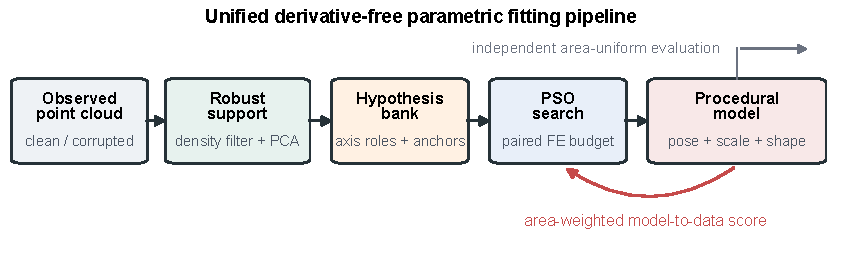
\includegraphics[width=\textwidth]{figures/pipeline.pdf}
\caption{Fitting pipeline.  Representation, support construction, initialization,
optimizer, and independent evaluation are varied or audited separately.}
\label{fig:pipeline}
\end{figure*}

Let $\mathcal D=\{\mathbf d_j\}_{j=1}^{N}\subset\R^3$ be the observation and
$\mathcal M(\boldsymbol\theta)=\{\mathbf m_i(\boldsymbol\theta)\}_{i=1}^{K}$
the surface sampled from a procedural rule.  The fitting problem is
\begin{equation}
\boldsymbol\theta^*=\arg\max_{\boldsymbol\theta\in\Theta}
S\!\left(\mathcal M(\boldsymbol\theta),\mathcal D\right).
\end{equation}
All optimizers act on normalized vectors in $[-1,1]^p$ and share the same
affine decoder and physical bounds.

\subsection{PMF-Style Partial Cylinder}
The seven cylinder parameters are the base point
$(x_0,y_0,z_0)$, radius $r$, height $h$, start angle $\alpha$, and positive
angular span $\beta$.  The lateral surface is
\begin{equation}
\mathbf c(u,z)=
\begin{bmatrix}
x_0+r\cos u\\ y_0+r\sin u\\ z
\end{bmatrix},
\end{equation}
where $u\in[\alpha,\alpha+\beta]$ and $z\in[z_0,z_0+h]$.
We optimize the span rather than two unordered endpoint angles.  Midpoint
sampling avoids a duplicated seam.  The synthetic task matches the dimensional
structure of PMF model M5, but the generated point clouds are a reconstruction
and are not the original D5/D6 data from~\cite{zhang2019pmf}.

\subsection{Posed Superquadric Rule}
The superquadric parameter vector contains translation, three positive scales,
two exponents, and XYZ Euler angles,
\begin{equation}
\boldsymbol\theta=[\mathbf t^{\mathsf T},\mathbf a^{\mathsf T},e_1,e_2,
\boldsymbol\varphi^{\mathsf T}]^{\mathsf T}\in\R^{11}.
\end{equation}
With $C(v,e)=\operatorname{sgn}(\cos v)|\cos v|^e$ and
$S(v,e)=\operatorname{sgn}(\sin v)|\sin v|^e$, its local surface is
\begin{equation}
\mathbf q(\eta,\omega)=
\begin{bmatrix}
a_1C(\eta,e_1)C(\omega,e_2)\\
a_2S(\eta,e_1)C(\omega,e_2)\\
a_3S(\omega,e_2)
\end{bmatrix}.
\end{equation}
The posed point is $\mathbf R(\boldsymbol\varphi)\mathbf q+\mathbf t$.
The periodic $\eta$ grid excludes its endpoint, and the two exact poles are
displaced by $10^{-4}$ to avoid duplicate samples.

\subsection{Directed Mean-Measure Score}
For every sampled model point, let
\begin{equation}
r_i=\min_{\mathbf d\in\mathcal D}\|\mathbf m_i-\mathbf d\|_2.
\end{equation}
If $\bar r$ is the model-to-data mean, $\delta$ is the input resolution, and
$A(\boldsymbol\theta)$ is the sampled model measure, the implemented mean
measure is
\begin{equation}
S_{\mathrm{MM}}=\frac{A(\boldsymbol\theta)^{\rho}}
{\bar r/\delta+\varepsilon},\qquad \rho=0.5.
\label{eq:mm}
\end{equation}
The partial-cylinder study uses this directed term without data coverage.  The
closed-superquadric configuration additionally multiplies it by the fraction of
supported observations within $5\delta$.  These are declared configuration
choices; objective scores are never compared across estimator variants.

\subsection{Area-Consistent Quadrature}
Uniform increments in $(\eta,\omega)$ are not uniform in physical area.  We
split every periodic grid quadrilateral into two triangles and assign one third
of each triangle area to its incident vertices, producing nonnegative weights
$w_i$.  The weighted residual and numerical area are
\begin{equation}
\bar r_A=\frac{\sum_i w_i r_i}{\sum_i w_i},\qquad
\widehat A=\sum_i w_i.
\end{equation}
The ablation keeps candidate points and $\widehat A$ fixed and changes only the
residual average.  External evaluation is independent: it samples triangles in
proportion to area and then draws uniform barycentric points.

\subsection{Adaptive Density Support}
Gross outliers can enlarge bounds and alter $\delta$ before the directed score
is evaluated.  For each observation we compute its 16-nearest-neighbor distance
$d_i^{(16)}$ and cluster $\log(d_i^{(16)}+\varepsilon)$ into two groups by
deterministic $k$-means.  The group with the smaller median distance is retained.
Nearest-neighbor local density is a classical cue for unsupervised outlier
detection~\cite{breunig2000lof}; our rule is a simpler one-dimensional split,
not the LOF score.
No contamination fraction or ground-truth label is supplied.  Labels are used
only after selection to audit precision and recall.  On the reconstructed
cylinder, the rule retains 2,056 of 4,096 points at 50\% outliers and 2,050 of
10,240 at 80\%, with inlier precision/recall above 0.993 in both conditions.
This mechanism assumes that inliers form a denser surface population than the
volume outliers; it is not a guarantee for arbitrary adversarial contamination.

\subsection{Geometry-Guided PSO Initialization}
For posed superquadrics, robust center, principal axes, and quantile extents
define a bank of axis-role hypotheses.  Seventy-five percent of particles are
drawn as jittered variants of this bank and the remainder uniformly from the
full bounds.  The optimizer and objective are otherwise unchanged.  Under the
20\% outlier condition, a fixed 75\% nearest-neighbor-density support is used
only to construct the initial hypotheses; the estimator still receives the
complete observation.  This distinction prevents an initialization gain from
being mislabeled as estimator robustness.  A post-selection audit over all
nine preregistered cases finds 1.000 inlier precision and 0.9375 inlier recall:
each 3,750-point support contains no generated volume outlier.  This perfect
separation is specific to the controlled uniform-volume outlier process and is
not evidence for arbitrary clustered or adversarial contamination.

\subsection{Template-Guided Character Initialization}
The character rule deforms a motor-program template through a bounded action
vector.  Its zero action therefore reproduces the undeformed candidate
template.  For the template-guided PSO ablation, half of the 16 particles
comprise the exact zero action and Gaussian perturbations with standard
deviation 0.15 in normalized action coordinates; the other half are sampled
uniformly from the full bounds.  The same construction is applied independently
to PSO and CS; their objectives, update equations, FE budgets, and candidate
templates are unchanged.  The resulting $2\times2$ design separates optimizer
choice from template-guided initialization rather than proposing a new
optimizer.

\section{Experimental Protocol}
\begin{figure*}[t]
\centering
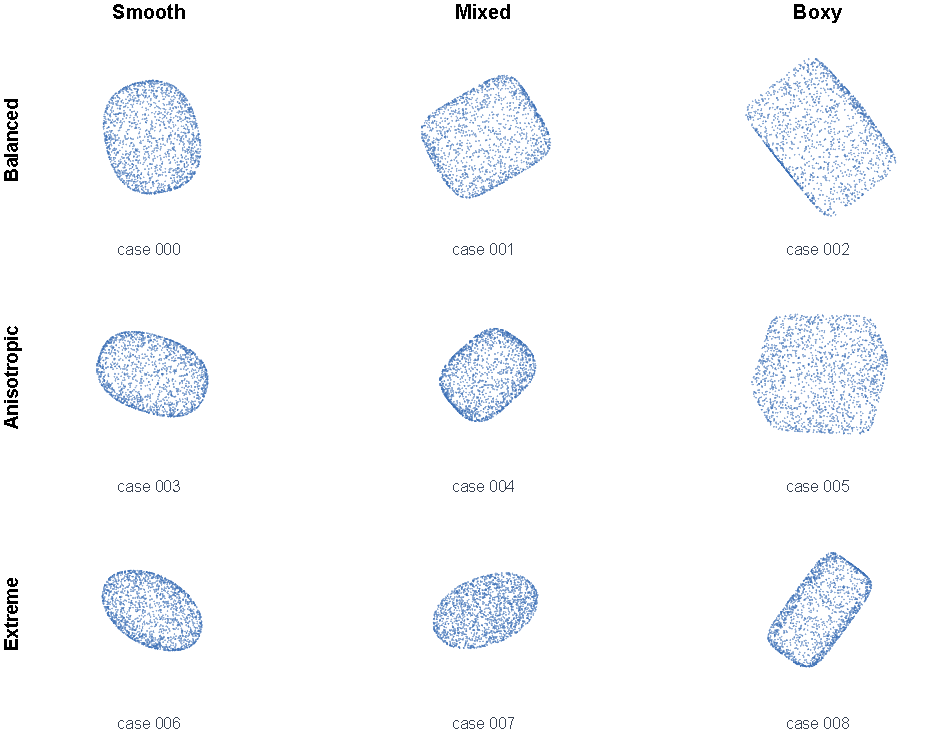
\includegraphics[width=\textwidth]{figures/stratified_superquadrics.pdf}
\caption{The first randomized $3\times3$ superquadric block used for controlled
recovery.  Columns vary shape and rows vary aspect-ratio regime.}
\label{fig:strata}
\end{figure*}

\subsection{Datasets and Corruptions}
The partial-cylinder reference contains 2,048 points sampled uniformly in
angle and height.  Contaminated sets preserve every clean point exactly and add
uniform-volume outliers to obtain 50\% and 80\% outlier ratios.  Kolmogorov--
Smirnov checks do not reject angular or height uniformity ($p=0.490$ and
$p=0.881$).

We additionally reconstruct the PMF M1 one-parameter similarity experiment.
The complete surface D1 and two nested partial observations D2 and D4 retain
100\%, 75\%, and 25\% of 12,288 regularly sampled points, respectively.  This
reconstruction tests whether weighted mean measure (WMM) preserves the optimum
under missing support; it is not presented as the authors' original PMF data.

The superquadric benchmark contains 30 randomly parameterized convex surfaces.
Shape exponent and aspect-ratio strata form repeated $3\times3$ blocks.  Every
case includes a clean observation, Gaussian noise with standard deviation 1\%
of the reference bounding-box diagonal, 20\% gross outliers, a random subset
retaining 20\% of points, and a spatially coherent cap retaining 20\% of the
surface.  Random sparsity and spatial occlusion are reported separately.  The
confirmatory controlled study uses all 30 cases; Fig.~\ref{fig:strata} shows
cases 000--008 as the first complete stratum block.
For an external qualitative test, we use the ModelNet40 test mesh
\texttt{bottle\_0338} from~\cite{wu2015modelnet}.  A 5,000-point area-sampled
observation is fitted and
evaluated against an independently sampled 20,000-point reference.  Because the
object is not generated by a superquadric, this test measures single-primitive
approximation rather than parameter recovery.

The character check uses the available Python-converted motor programs and
105$\times$105 images from the PMF character assets.  Ten available matched
template--observation pairs are fitted under 60\% salt-and-pepper corruption.
A $2\times2$ factorial comparison applies vanilla or template-guided
initialization to PSO and CS, with three paired-seed repeats for every matched
case and method.
A separate four-class experiment uses the complete run-1 subset: each of four
noisy observations is fitted against all four candidate templates, and the
candidate with the largest final PMF similarity is selected.  Three paired
optimization repeats are used for every observation--candidate cell.  This is a
closed-set fit-and-select experiment, not a full Omniglot recognition benchmark.

\subsection{Budgets, Pairing, and Metrics}
The main cylinder comparison uses population 80, 50,000 FEs, and 20 paired
seeds.  Its budget study uses five new paired seeds at 50,000, 199,920, and
499,920 FEs.  The latter values satisfy the exact PSO--CS population accounting
$80+160k$.  The density-support ablation uses five additional paired seeds per
condition and holds PSO and the 50,000-FE budget fixed.

The host exposes an RTX 5060 through CUDA.  The main PMF comparison, support
ablations, and superquadric robustness matrix use the preregistered CPU scoring
path: PSO and CS maintain NumPy populations and the mean-measure estimator uses
scikit-learn KDTree.  Before the budget-sensitivity study, a PyTorch-CUDA
candidate passed a numerical-equivalence gate but lost a paired 8,080-FE
end-to-end timing gate to CPU KDTree in all four optimizer--condition cells.
The budget study therefore also uses a shared scikit-learn backend.  In every
study, publication metrics are independently recomputed with the CPU
nearest-neighbor stack; wall-time comparisons are made only within a shared
backend.

Guided PSO uses population 16 and 10,000 FEs on each superquadric condition.
Its inertia decreases linearly from 0.9 to 0.4, following the modified-PSO
design of Shi and Eberhart~\cite{shi1998modified}.
Three seeds are paired within each of the 30 independently generated cases;
cases 000--008 reuse the same three seeds from the earlier five-seed matrix.
EMS uses its documented
iterative stopping settings and is an accuracy reference rather than an
FE-matched optimizer.  All recovery metrics are recomputed against an analytic
clean surface using 20,000 area-uniform reference points and 20,000 independently
sampled fitted points.  Symmetric Chamfer distance~\cite{fan2017pointset} is
the primary recovery metric.  Superquadric success is predefined as distance
at most 0.05; the cylinder threshold is derived once from the clean reference
resolution and is then fixed for every condition.  We report medians, IQRs,
success counts, paired wins, and exact two-sided Wilcoxon signed-rank tests.
Audited per-case summaries additionally retain minima, maxima, and success
counts at 0.04, 0.05, and 0.06, because a minority parameter basin can lie
outside the IQR.
The exact distribution is obtained by enumerating all signs of the nonzero
average ranks; zero differences and tied absolute ranks are retained explicitly
in the audit record rather than triggering an asymptotic fallback.

The character study likewise uses population 16 and exactly 10,000 FEs per
candidate.  PSO and CS use paired seeds and the same CPU nearest-neighbor
backend.  The ten-pair matched study has three paired-seed repeats per
case--method cell and reports both PMF similarity (higher is better) and an
independently recomputed symmetric Chamfer distance (lower is better).  Guided
effects are first paired within seed and then reduced to one median per case;
exact tests therefore use ten case-level values.  The four-way experiment also
has three stochastic repeats per observation--candidate cell.  Its signed class
margin is the true-template score minus the largest competing-template score.
For inference, the three margins are first reduced to one median per
observation, and exact paired tests use the resulting four observation-level
values; optimization repeats are not treated as independent character classes.

\FloatBarrier
\section{Results}
\subsection{PMF-Style Partial-Similarity Sanity Check}
Figure~\ref{fig:m1} reproduces the mechanism behind PMF's simple M1 task using
the reconstructed observations defined above.  WMM places the maximizer at
$\hat\theta=0.98$ for D1, D2, and D4, within 0.02 of the target
$\theta=1$.  The unweighted mean measure has the same clean maximizer but drifts
to 0.77 at 75\% support and 0.01 at 25\% support.  This controlled result
validates the missing-support weighting before optimizer comparisons; it does
not substitute for a run on the original author files.

\begin{figure*}[t]
\centering
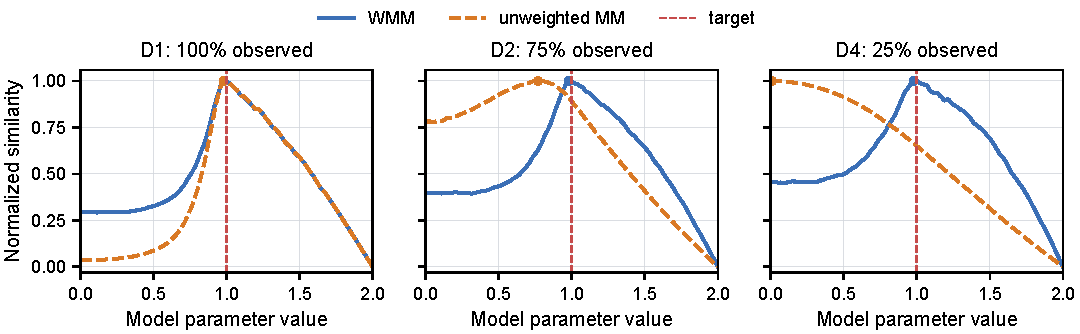
\includegraphics[width=.94\textwidth]{figures/pmf_m1_partial_similarity.pdf}
\caption{Reconstructed PMF M1 similarity curves.  WMM retains the target
optimum under partial observations, whereas the unweighted measure increasingly
favors undersized models.}
\label{fig:m1}
\end{figure*}

\subsection{Noisy Character Fitting and Four-Way Repeats}
The audited matched factorial contains \CharacterFactorialCells{} completed
fits with no failed cells.  Template guidance increases the case-level median
PMF similarity by \CharacterFactorialPSOSimilarityGain{} for PSO, with positive
effects in \CharacterFactorialPSOSimilarityWins{} cases and an exact paired
test of $p=\CharacterFactorialPSOSimilarityP$.  For CS, the corresponding gain
is \CharacterFactorialCSSimilarityGain{}, with
\CharacterFactorialCSSimilarityWins{} positive cases and
$p=\CharacterFactorialCSSimilarityP$.  The external geometric endpoint is more
qualified: median Chamfer reductions are only
\CharacterFactorialPSOChamferReduction{} for PSO and
\CharacterFactorialCSChamferReduction{} for CS, both positive in 6/10 cases,
with $p=\CharacterFactorialPSOChamferP$ and
$p=\CharacterFactorialCSChamferP$, respectively.  Thus the shared warm start
improves search according to the fitted objective, but these data do not
establish a Chamfer improvement.

Figure~\ref{fig:characterdimension} tests the proposed dimensional explanation
descriptively.  Similarity gain is not positively associated with action
dimension for PSO ($\rho=\CharacterFactorialPSODimensionRho$), whereas CS shows
a positive association ($\rho=\CharacterFactorialCSDimensionRho$).  This
optimizer-specific pattern does not support a general claim that higher
dimension necessarily benefits more from guidance.

The repeated four-way fit-and-select experiment exposes a more specific failure
mode (Table~\ref{tab:character4way}).  Vanilla PSO misclassifies observation 1
in two of three repeats.  Its correct candidate has the largest action
dimension (56 versus 46, 43, and 31 for the alternatives).  Template-guided PSO
removes both observed failures, changing the aggregate result from
\CharacterVanillaAccuracy{} (\CharacterVanillaAccuracyPercent) to
\CharacterGuidedAccuracy{} (\CharacterGuidedAccuracyPercent) with a median
signed true-class margin of \CharacterGuidedMarginMedian{}.  CS obtains
\CharacterCSAccuracy{} (\CharacterCSAccuracyPercent) and fails once on
observation 4, whereas Guided CS obtains \CharacterGuidedCSAccuracy{}
(\CharacterGuidedCSAccuracyPercent) with median margin
\CharacterGuidedCSMarginMedian{}.  Both within-optimizer comparisons therefore
favor guided initialization descriptively.  After reducing repeats to one
median margin per observation, the exact paired tests give
$p=\CharacterGuidedPSOVsVanillaPSOP$ for Guided versus vanilla PSO and
$p=\CharacterGuidedCSVsVanillaCSP$ for Guided versus vanilla CS.  Guided PSO
versus Guided CS gives $p=\CharacterGuidedPSOVsGuidedCSP$.  With four
observation-level pairs, these tests cannot establish population-level
recognition superiority.

\begin{table}[!b]
\caption{Repeated four-way noisy-character fit-and-select results.  Each repeat
contains four class decisions; displayed margins are pooled over 12 decisions,
whereas inferential tests first aggregate repeats within observation.}
\label{tab:character4way}
\centering
\begin{tabular}{lrrrrr}
\toprule
Method & R1 & R2 & R3 & Total & Med. margin \\
\midrule
Vanilla PSO & 3/4 & 3/4 & 4/4 & \CharacterVanillaAccuracy
            & \CharacterVanillaMarginMedian \\
Guided PSO & 4/4 & 4/4 & 4/4 & \CharacterGuidedAccuracy
           & \CharacterGuidedMarginMedian \\
CS & 4/4 & 4/4 & 3/4 & \CharacterCSAccuracy
   & \CharacterCSMarginMedian \\
Guided CS & 4/4 & 4/4 & 4/4 & \CharacterGuidedCSAccuracy
          & \CharacterGuidedCSMarginMedian \\
\bottomrule
\end{tabular}
\end{table}

\begin{figure*}[t]
\centering
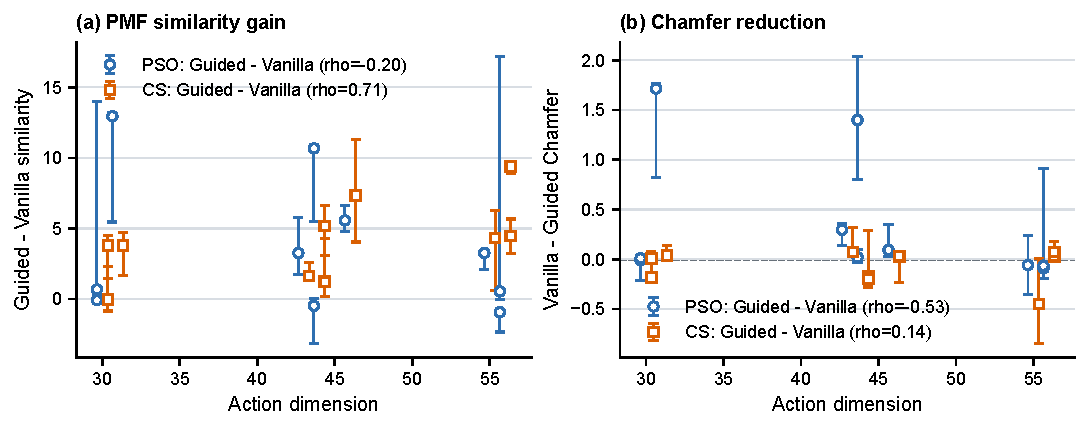
\includegraphics[width=.94\textwidth]{figures/character_dimension_effect.pdf}
\caption{Template-guidance effects across ten noisy-character cases.  Each
point is the median guided-minus-vanilla paired effect over three seeds; error
bars show the paired-effect IQR.  Positive values favor guidance for both
metrics.  Spearman $\rho$ is descriptive; exact tests use one aggregate per
case.  Internal similarity gains are stronger than external Chamfer gains.}
\label{fig:characterdimension}
\end{figure*}

\begin{figure*}[t]
\centering
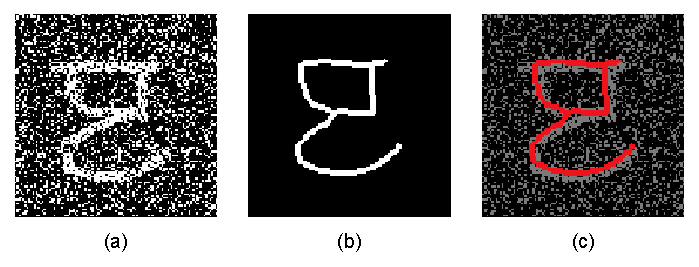
\includegraphics[width=.76\textwidth]{figures/character_fit_example_pmf_style.pdf}
\caption{A successful noisy-character fit in the visual convention of PMF.
Case r7-t1 has the lowest Guided-PSO case-median Chamfer among the ten audited
cases; the displayed repeat is its median-Chamfer run (2.919) across three
seeds.  Panels show (a) the complete corrupted observation, (b) the fitted
motor-program centerline, and (c) the fitted centerline overlaid in red.
Centerline thinning and display-width dilation are used only for visualization;
fitting and reported metrics use the original rendered occupancy.}
\label{fig:characterexample}
\end{figure*}

\subsection{Optimizer Choice on the Partial Cylinder}
Table~\ref{tab:optimizer} and Fig.~\ref{fig:pmf} show that PSO is substantially
more reliable under the fixed clean-input FE budget.  It wins
\PMFCleanPSOWins{} paired runs and the exact test gives
$p=\PMFCleanWilcoxonP$.  Under 50\% unfiltered
outliers, however, neither optimizer is reliable: PSO succeeds in only
\PMFOutlierFiftyPSOSuccess{} and CS in \PMFOutlierFiftyCSSuccess{}, while their
paired Chamfer difference is not significant ($p=\PMFOutlierFiftyWilcoxonP$).
Thus the clean result supports optimizer selection, not a claim that PSO alone
provides outlier robustness.

\begin{table}[t]
\caption{PSO--CS cylinder comparison at 50,000 FEs (20 paired runs).}
\label{tab:optimizer}
\centering
\begin{tabular}{llcc}
\toprule
Condition & Method & Median CD & Success \\
\midrule
Clean & PSO & \PMFCleanPSOMedian & \PMFCleanPSOSuccess \\
      & CS  & \PMFCleanCSMedian  & \PMFCleanCSSuccess \\
50\% outliers & PSO & \PMFOutlierFiftyPSOMedian & \PMFOutlierFiftyPSOSuccess \\
              & CS  & \PMFOutlierFiftyCSMedian  & \PMFOutlierFiftyCSSuccess \\
\bottomrule
\end{tabular}
\end{table}

\begin{figure*}[t]
\centering
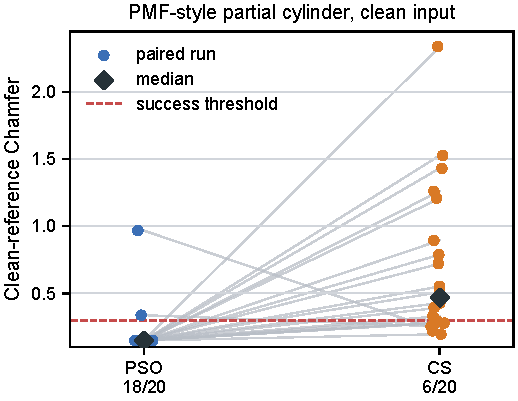
\includegraphics[width=.47\textwidth]{figures/pmf_clean_paired.pdf}\hfill
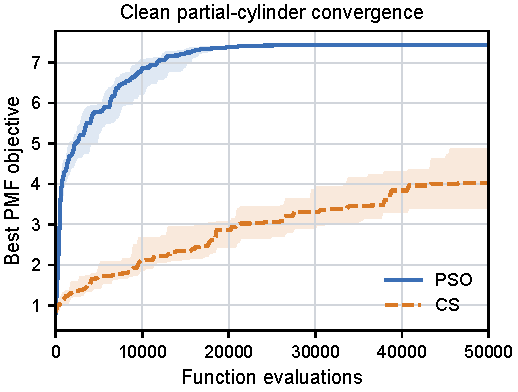
\includegraphics[width=.47\textwidth]{figures/pmf_clean_convergence.pdf}
\caption{Clean partial-cylinder comparison.  Left: paired external recovery
errors; right: median and IQR of the best internal objective versus FEs.}
\label{fig:pmf}
\end{figure*}

\ifdefined\BudgetFiftyKCleanPSOMedian
\subsection{Function-Evaluation Budget Sensitivity}
Table~\ref{tab:budget} and Fig.~\ref{fig:budget} separate optimizer ranking from
budget starvation.  The three budgets preserve exact PSO--CS accounting for a
population of 80.  Comparisons at each budget use five new paired seeds, and
the endpoint tests pair 50,000 and 499,920 FEs within each optimizer.  On clean
input the endpoint exact tests give $p=\BudgetCleanPSOEndpointP$ for PSO and
$p=\BudgetCleanCSEndpointP$ for CS; under 50\% outliers they give
$p=\BudgetOutlierFiftyPSOEndpointP$ and
$p=\BudgetOutlierFiftyCSEndpointP$, respectively.  These five-pair tests are
reported with their limited attainable resolution rather than used alone to
declare an optimizer universally superior.

\begin{table}[t]
\caption{PMF-cylinder budget sensitivity (five paired runs per cell).}
\label{tab:budget}
\centering
\begin{tabular}{lrrrr}
\toprule
Condition & FEs & PSO CD & CS CD & Succ. P/C \\
\midrule
Clean & 50,000  & \BudgetFiftyKCleanPSOMedian
                    & \BudgetFiftyKCleanCSMedian
                    & \BudgetFiftyKCleanPSOSuccess/\BudgetFiftyKCleanCSSuccess \\
      & 199,920 & \BudgetTwoHundredKCleanPSOMedian
                    & \BudgetTwoHundredKCleanCSMedian
                    & \BudgetTwoHundredKCleanPSOSuccess/\BudgetTwoHundredKCleanCSSuccess \\
      & 499,920 & \BudgetFiveHundredKCleanPSOMedian
                    & \BudgetFiveHundredKCleanCSMedian
                    & \BudgetFiveHundredKCleanPSOSuccess/\BudgetFiveHundredKCleanCSSuccess \\
50\% out. & 50,000  & \BudgetFiftyKOutlierFiftyPSOMedian
                       & \BudgetFiftyKOutlierFiftyCSMedian
                       & \BudgetFiftyKOutlierFiftyPSOSuccess/\BudgetFiftyKOutlierFiftyCSSuccess \\
         & 199,920 & \BudgetTwoHundredKOutlierFiftyPSOMedian
                       & \BudgetTwoHundredKOutlierFiftyCSMedian
                       & \BudgetTwoHundredKOutlierFiftyPSOSuccess/\BudgetTwoHundredKOutlierFiftyCSSuccess \\
         & 499,920 & \BudgetFiveHundredKOutlierFiftyPSOMedian
                       & \BudgetFiveHundredKOutlierFiftyCSMedian
                       & \BudgetFiveHundredKOutlierFiftyPSOSuccess/\BudgetFiveHundredKOutlierFiftyCSSuccess \\
\bottomrule
\end{tabular}
\end{table}

\begin{figure*}[t]
\centering
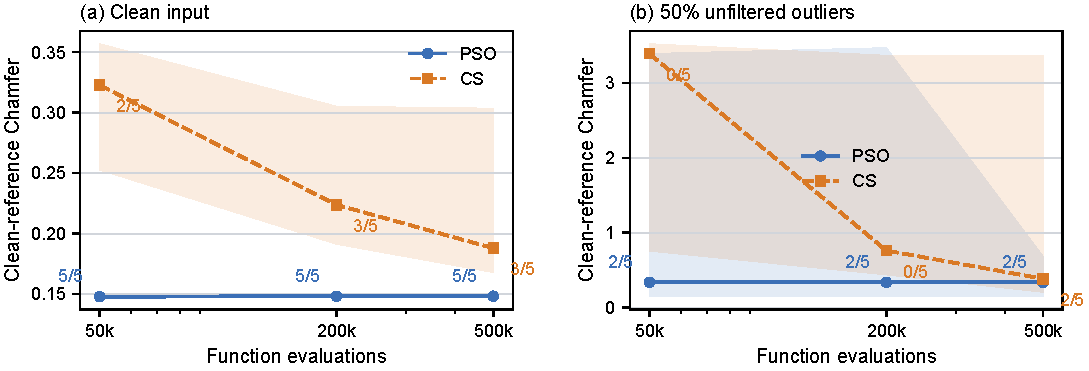
\includegraphics[width=.94\textwidth]{figures/pmf_budget_sensitivity.pdf}
\caption{Median and IQR of external Chamfer versus function-evaluation budget;
labels give successes among five paired runs.}
\label{fig:budget}
\end{figure*}
\fi

\subsection{Support-Set Ablation}
Adaptive support trades a small clean-data penalty for a large change in
breakdown behavior (Table~\ref{tab:support}, Fig.~\ref{fig:support}).  Both clean
variants succeed in 5/5 runs, but the median CD increases from
\SupportCleanFullMedian{} to \SupportCleanAdaptiveMedian{}.  At 50\% and 80\%
outliers, adaptive support succeeds in every run with median CD near 0.149,
whereas full-input success is 1/5 and 0/5.  With only five pairs, the exact
$p$-values are \SupportOutlierFiftyWilcoxonP{} and
\SupportOutlierEightyWilcoxonP{}; the 80\% value 0.0625 is the smallest attainable
two-sided exact value for five nonzero differences.  We therefore report the
complete success separation and effect size without calling it significant at
0.05.

\begin{table}[t]
\caption{Density-support ablation with PSO (five paired runs).}
\label{tab:support}
\centering
\begin{tabular}{lcccr}
\toprule
Condition & \multicolumn{2}{c}{Full input} & \multicolumn{2}{c}{Adaptive}\\
 & CD & Succ. & CD & Succ.\\
\midrule
Clean & \SupportCleanFullMedian & \SupportCleanFullSuccess
      & \SupportCleanAdaptiveMedian & \SupportCleanAdaptiveSuccess\\
50\% & \SupportOutlierFiftyFullMedian & \SupportOutlierFiftyFullSuccess
     & \SupportOutlierFiftyAdaptiveMedian & \SupportOutlierFiftyAdaptiveSuccess\\
80\% & \SupportOutlierEightyFullMedian & \SupportOutlierEightyFullSuccess
     & \SupportOutlierEightyAdaptiveMedian & \SupportOutlierEightyAdaptiveSuccess\\
\bottomrule
\end{tabular}
\end{table}

\begin{figure}[t]
\centering
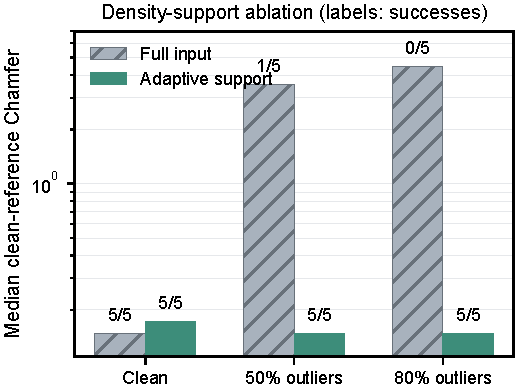
\includegraphics[width=\columnwidth]{figures/density_support_ablation.pdf}
\caption{Median clean-reference Chamfer on a logarithmic scale.  Labels show
successes among five paired runs.}
\label{fig:support}
\end{figure}

\subsection{Initialization and Area Weighting}
Guided initialization improves the box and cylinder canonical tasks from 1/5
to 5/5 successes, reducing median CD from \InitBoxRandomMedian{} to
\InitBoxGuidedMedian{} and from \InitCylinderRandomMedian{} to
\InitCylinderGuidedMedian{}.  The already-easy ellipsoid remains 5/5 with
essentially unchanged median error.  Area weighting is mixed: it improves the
box and ellipsoid medians but slightly worsens the cylinder median.  It should
therefore be interpreted as area-consistent quadrature, not a universally
better stochastic objective.

\begin{figure*}[t]
\centering
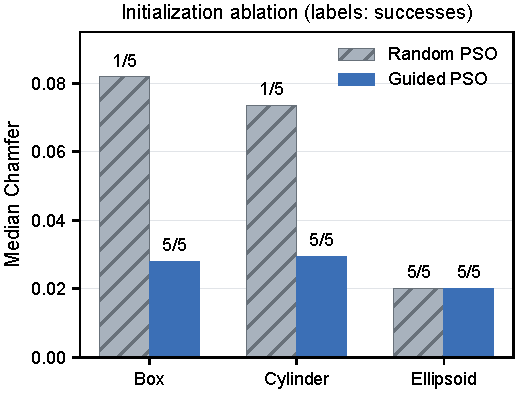
\includegraphics[width=.47\textwidth]{figures/guided_initialization_ablation.pdf}\hfill
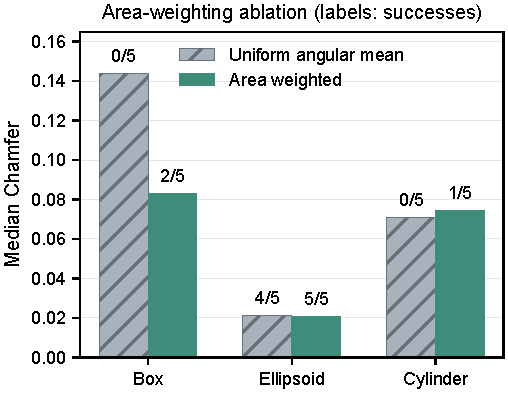
\includegraphics[width=.47\textwidth]{figures/area_ablation.pdf}
\caption{Canonical-shape ablations.  Left: random versus guided PSO
initialization; right: uniform angular mean versus area-weighted residual.}
\label{fig:ablations}
\end{figure*}

\subsection{Clean Randomized Superquadrics and EMS}
Across \SQRunsPerCondition{} Guided-PSO runs on \SQIndependentCases{} clean
randomized cases, the run-level
median CD is \SQRandomPSOMedian{} and \SQRandomPSOSuccess{} runs succeed.  EMS
succeeds in \SQRandomEMSSuccess{} deterministic fits with median CD
\SQRandomEMSMedian{}, wins \SQRandomEMSWins{} paired cases, and gives
$p=\SQRandomWilcoxonP$.  This is an
important negative result: the general derivative-free extension can fit posed
superquadrics, but it does not exceed the specialized solver on clean recovery.
On the 30 coherent 80\%-missing caps, EMS succeeds in
\EMSOcclusionSuccess{} cases, demonstrating that severe spatial occlusion is
also nontrivial for the dedicated method.

\subsection{Actual-Object Superquadric Approximation}
Figure~\ref{fig:modelnet} shows a fitted superquadric on an external ModelNet40
bottle point cloud.  Guided PSO reaches reference CD 0.02509 and
$F$-score@0.01 of 0.6842 using 10,000 FEs.  The overlay and distance map show
that one primitive captures the object's dominant elongated body while leaving
larger residuals near non-superquadric end structure.  This is evidence that
the implementation can operate on a real object mesh-derived point cloud, not
a claim that the bottle is exactly superquadric or that this single example
establishes dataset-level generalization.

\begin{figure*}[t]
\centering
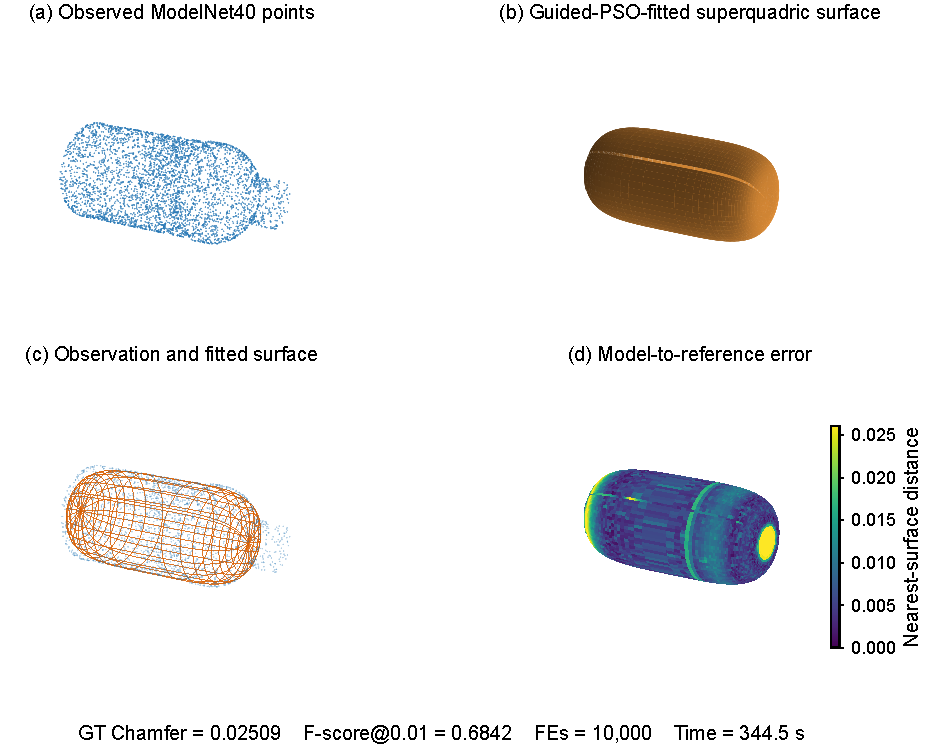
\includegraphics[width=.92\textwidth]{figures/modelnet40_bottle0338_pso.pdf}
\caption{Actual-object approximation on ModelNet40 \texttt{bottle\_0338}:
(a) observed points, (b) Guided-PSO-fitted superquadric, (c) overlay, and
(d) nearest-reference surface error.  Metrics use an independent 20,000-point
reference sample.}
\label{fig:modelnet}
\end{figure*}

\ifdefined\SQOcclusionPSOMedian
\subsection{Stratified Superquadric Robustness}
Table~\ref{tab:sqrobust} reports random sparsity and spatial occlusion
separately.  It gives descriptive Guided-PSO medians and success counts over all
\SQRunsPerCondition{} runs per condition.  Case-balanced analyses first take
the three-run median within each case and then summarize the
\SQIndependentCases{} case values; deterministic EMS statistics use the same
cases.  Paired degradation and inferential tests likewise pair each corrupted
case median with its own clean case median.  Thus stochastic repeats are not
treated as independent shape instances.  Absolute success
and paired degradation are complementary: a case can remain above the recovery
threshold yet show little corruption-induced loss if it was already difficult
on clean input.

\begin{table}[t]
\caption{Audited superquadric robustness results.}
\label{tab:sqrobust}
\centering
\begin{tabular}{lrrrr}
\toprule
Condition & PSO CD & Succ. & EMS CD & Succ. \\
\midrule
Clean & \SQRandomPSOMedian & \SQRandomPSOSuccess
      & \SQRandomEMSMedian & \SQRandomEMSSuccess \\
1\% noise & \SQNoisePSOMedian & \SQNoisePSOSuccess
           & \SQNoiseEMSMedian & \SQNoiseEMSSuccess \\
20\% outliers & \SQOutlierPSOMedian & \SQOutlierPSOSuccess
               & \SQOutlierEMSMedian & \SQOutlierEMSSuccess \\
80\% random missing & \SQRandomMissingPSOMedian & \SQRandomMissingPSOSuccess
                     & \SQRandomMissingEMSMedian & \SQRandomMissingEMSSuccess \\
80\% cap occlusion & \SQOcclusionPSOMedian & \SQOcclusionPSOSuccess
                    & \SQOcclusionEMSMedian & \SQOcclusionEMSSuccess \\
\bottomrule
\end{tabular}
\end{table}

The Gaussian-noise result is not merely an artifact of the primary 0.05
success threshold: only \SQNoisePSOSuccessAtSix{} runs pass when the threshold
is relaxed to 0.06.  The preregistered shape strata localize the degradation:
smooth cases retain \SQNoiseSmoothSuccess{} successes, whereas boxy cases retain
\SQNoiseBoxySuccess{}.  Relative to each case's own clean median, the median
degradation is \SQNoiseRelativeDegradation{} and the exact paired test gives
$p=\SQNoisePairedCleanP$.  Parameter diagnostics keep the recovered centers and
symmetry-aware frames close to the references but show larger scale and
shape-exponent errors.  This pattern is consistent with noise-induced coupling
of sharp-region scale and exponent estimates, rather than a gross sampling or
translation failure.

Coherent 80\% cap occlusion is a systematic failure rather than an isolated
bad seed: Guided-PSO succeeds in \SQOcclusionPSOSuccess{} runs, even at the
relaxed 0.06 threshold.  In the original nine-case diagnostic block,
reconstructing the production bounds from each visible input shows that the
ground-truth center is outside the admissible box in
\SQOcclusionCenterInfeasible{} cases and inside it in
\SQOcclusionCenterFeasible{} cases; all scales remain admissible.  Bound
exclusion therefore explains part, but not all, of the result because the five
center-feasible cases also fail.  The remaining failures are consistent with
the ambiguity of extrapolating a whole symmetric surface from a one-sided cap
using a model-to-visible-data objective.  We report this limitation rather than
tuning the bounds after observing the test matrix.

\fi

\FloatBarrier
\section{Discussion}
The cylinder experiments isolate two mechanisms.  PSO reaches the narrow clean
optimum more reliably than CS at 50,000 FEs, but both fail when estimator inputs
are dominated by volume outliers.  Density support repairs the latter failure
without altering PSO.  It is therefore incorrect to attribute the 50\% or 80\%
gain to the optimizer.  Conversely, the clean penalty shows that filtering is
not free and should be enabled only when its density-separation assumption is
appropriate.

The superquadric study makes a second distinction.  A procedural rule and
black-box search provide breadth: the same infrastructure can represent many
posed shapes and can accept arbitrary differentiability.  EMS provides depth:
its likelihood model and switching procedure exploit superquadric-specific
structure and achieve better clean accuracy.  These methods should not be
presented as equivalent algorithms merely because both output superquadric
parameters.

The character experiment adds a complementary search observation.  Candidate
templates can have different action dimensions, so a fixed FE budget does not
imply equal coverage of their search spaces.  A semantically meaningful neutral
action removes all observed classification failures for both optimizers without
changing the score.  The complete $2\times2$ result therefore attributes the
shared improvement to initialization design.  Guided PSO has the larger pooled
median margin, but the four observation-level pairs do not establish that it is
superior to Guided CS.  The larger ten-case factorial strengthens the internal
score result for both optimizers, but its independent Chamfer tests remain
nonsignificant.  Moreover, only CS shows a positive descriptive relationship
between action dimension and similarity gain.  These disagreements illustrate
why objective value, geometry, and closed-set selection must remain separate
endpoints.

Finally, the internal objective, Chamfer against the corrupted input, and
Chamfer against the clean analytic reference answer different questions.  For
example, a correct 80\%-outlier fit has a contaminated-input Chamfer near 2.72
but a clean-reference Chamfer near 0.149.  Every success label and paper claim
uses the independently recomputed clean-reference metric.

\section{Limitations}
The 50\% and 80\% support results use uniform-volume outliers whose local
density differs strongly from the sampled surface; they do not establish
tolerance to clustered, structured, or adversarial outliers.  Moreover, 1\%
Gaussian perturbations degrade the low-exponent boxy stratum, so robustness to
sparse volume outliers does not imply noise robustness at sharp regions.  The
five paired support and ablation runs also limit exact-test resolution.
The character evidence remains limited to ten matched cases with three repeats
per cell, and the closed-set experiment contains only four observations.  The
case-level tests avoid pseudoreplication but have modest resolution, while the
action-dimension correlations are descriptive and confounded with character
identity.  Neither experiment estimates population recognition accuracy or
class-level generalization; those claims require additional character programs
and independent classes.
Euler-angle symmetries and axis permutations make raw parameter errors
ambiguous, so external surface error is the primary endpoint.  The cylinder
data reproduce a PMF-style task, not the original observations, and the
30-case synthetic superquadric matrix is a controlled benchmark rather than a
claim of broad real-world generalization.  Under coherent 80\% cap occlusion,
the nine-case bound audit excludes the true center in four cases; the other
five feasible cases expose partial-view identifiability limits.

\section{Conclusion}
This study treats optimizer choice and robust support construction as separate
design problems in parametric surface fitting.  PSO is more reliable than CS
under the same 50,000-FE budget on the clean reconstructed PMF cylinder, but
this advantage does not by itself handle gross contamination.  A label-free
nearest-neighbor-density split
restores recovery under the evaluated volume-outlier process, with an explicit
clean-data tradeoff.  The extension to posed superquadrics demonstrates the
generality of procedural search while the EMS comparison quantifies the cost of
that generality.  Across a separate character task, shared template guidance
improves the internal objective for both optimizers without yet demonstrating a
corresponding Chamfer improvement.  The results motivate separately auditing sampling,
preprocessing, search budgets, and independent evaluation instead of assigning
every gain to one optimizer.

\FloatBarrier
\bibliographystyle{IEEEtran}
\bibliography{references}

\end{document}
